
\renewcommand{\EntradaBibtex}{ConteoMonedasAppMovil_SistemasInteligentes_UPV_2023}

\begin{frame}{\citetitle{\EntradaBibtex} \footnotemark[1] (1)}
\begin{block}{Motivación} 
Se requiere migrar la aplicación móvil para conteo de monedas
\begin{itemize}
\item Utiliza la cámara del teléfono inteligente
\item Mismas limitantes de la aplicación de escritorio
\begin{itemize}
\item Las monedas pueden estar encimadas (con cierto grado permisible)
\item Se limitan a monedas de la misma denominación
\end{itemize}
\item Se emplean herramientas para eliminar ruido, detectar circulos
\item Por el momento el usuario solo puede seleccionar un\usepackage[symbol]{footmisc} denominación
\end{itemize}
\end{block} 
\footnotetext[1]{\fullcite{\EntradaBibtex}}
\end{frame}

\begin{frame}{\citetitle{\EntradaBibtex} (2)}

\begin{center}
	\begin{tabular}{cc}
		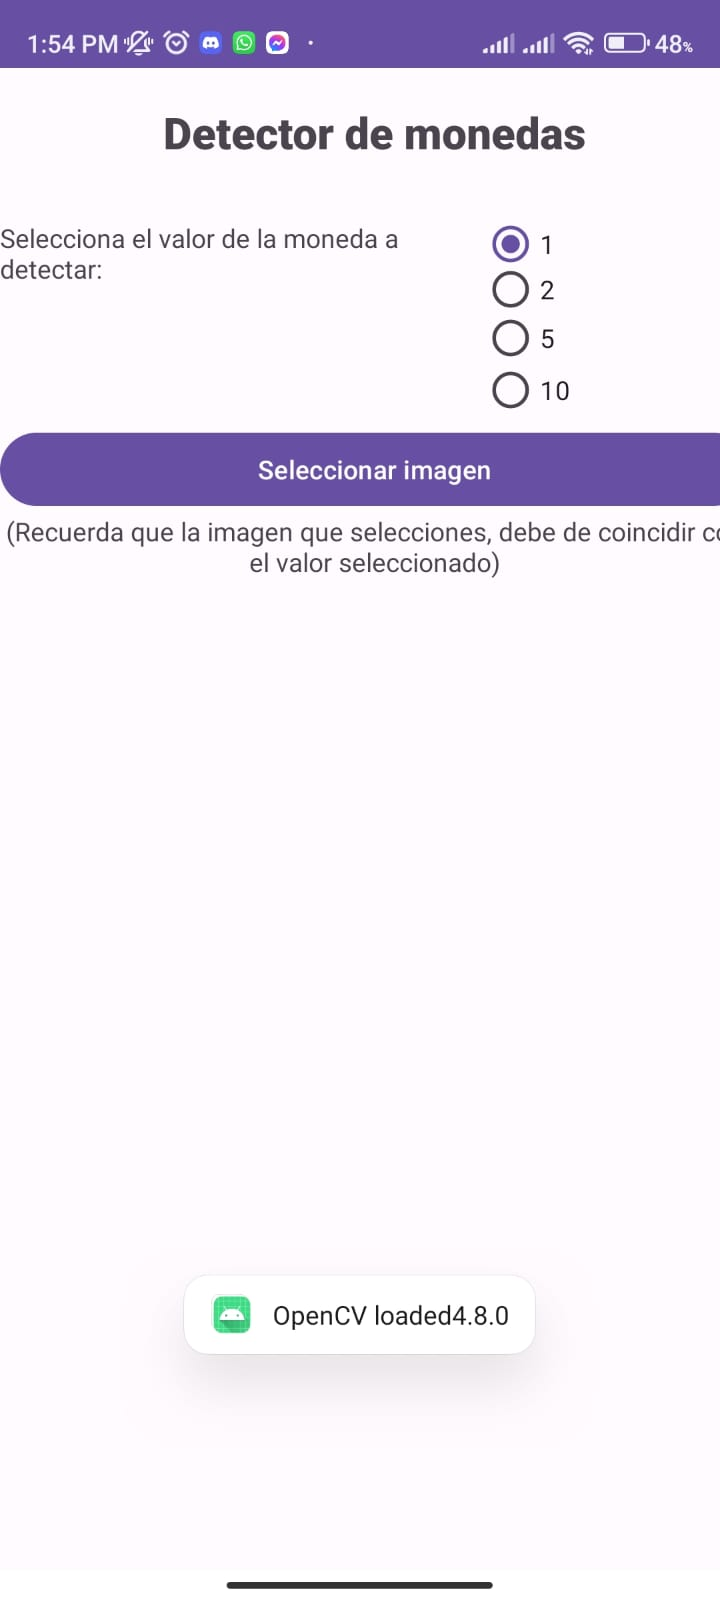
\includegraphics[width=0.28\linewidth]{2024_ConteoMonedasEscritorio/figs/1.jpeg} &
		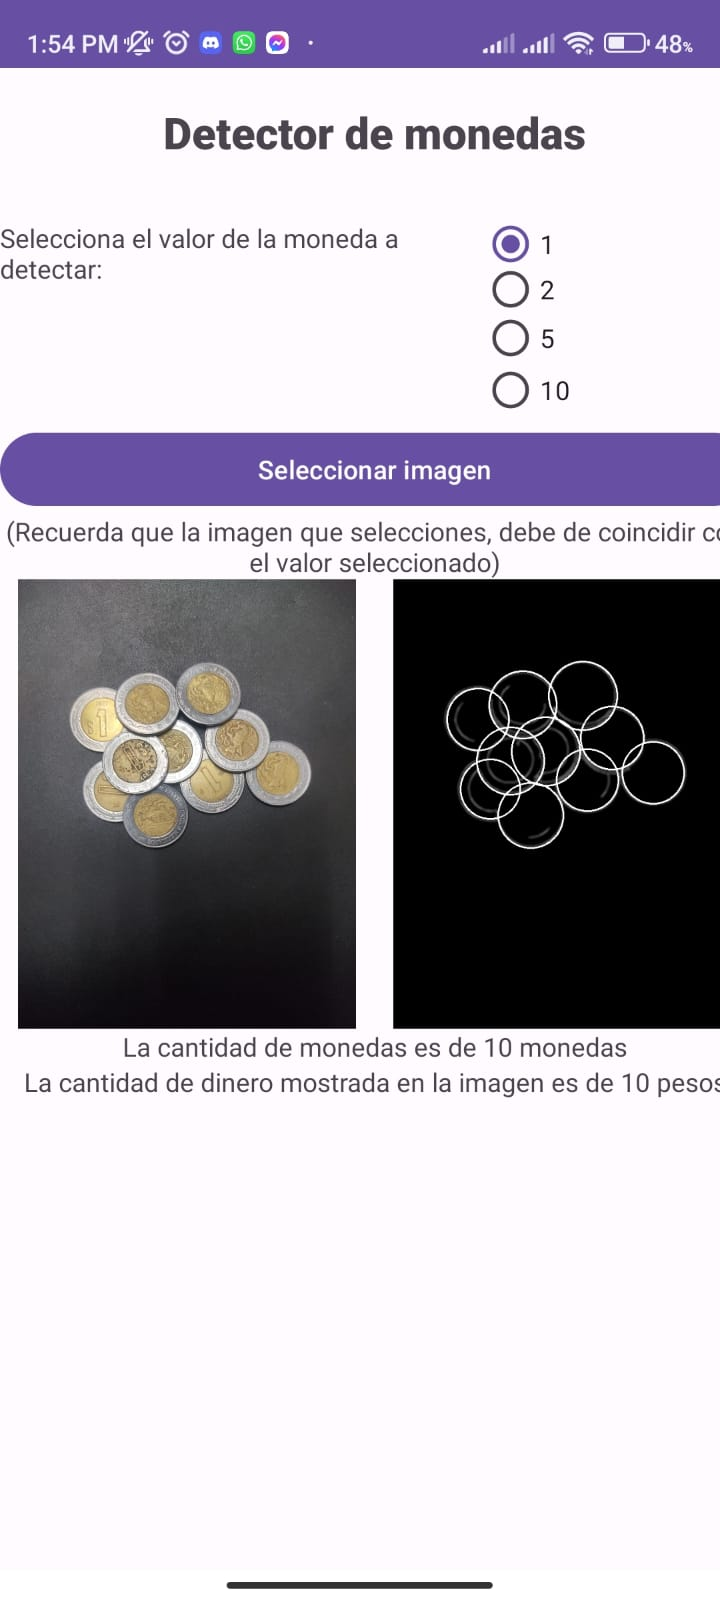
\includegraphics[width=0.28\linewidth]{2024_ConteoMonedasEscritorio/figs/4.jpeg} \\

	\end{tabular}
\end{center}
\end{frame}



\renewcommand{\EntradaBibtex}{ConteoMonedasEscritorio_SistemasInteligentes_UPV_2024}

\begin{frame}{\citetitle{\EntradaBibtex} \footnotemark[1] (1)}
\begin{block}{Motivación} 
Se requiere una herramienta para apoyar a pequeños comerciantes en el conteo de su morralla
\begin{itemize}
\item Se requiere una cámara WEB conectada a la computadora, montada en un tripie a cierta altura	
\item Por el momento se requieren condiciones muy particulares (fondo blanco, respectar distancia entre cámara-objetos)
\begin{itemize}
\item Las monedas pueden estar encimadas (con cierto grado permisible)
\end{itemize}
\item Se emplean herramientas para eliminar ruido, detectar circulos
\item Los circulos se ajustan por tamaño para determinar las denominaciones
\item Al final, se genra como resultado el estimado de la cantidad de dinero existente (no sólo el número de monedas)
\end{itemize}
\end{block} 
\footnotetext[1]{\fullcite{\EntradaBibtex}}
\end{frame}


\begin{frame}{\citetitle{\EntradaBibtex} (2)}
%\begin{block}{Pantallas Principales} 

%\begin{columns}
% Column 1
%\column{.8\linewidth}

\begin{center}
	\begin{tabular}{ccc}
		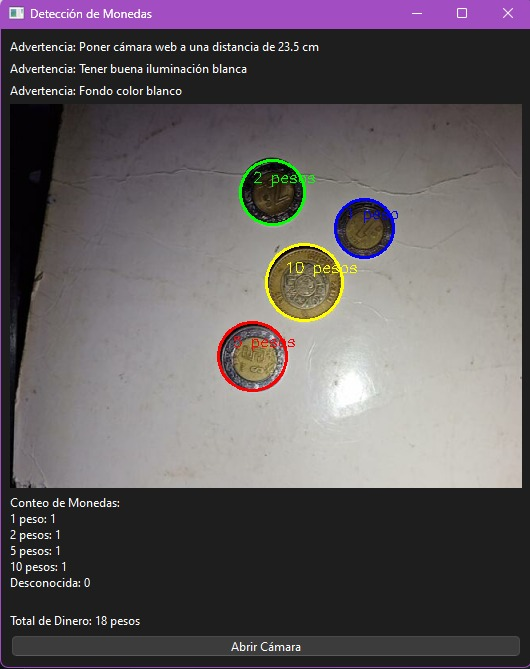
\includegraphics[width=0.32\linewidth]{2024_ConteoMonedasEscritorio/figs/ct1b.jpeg} &
		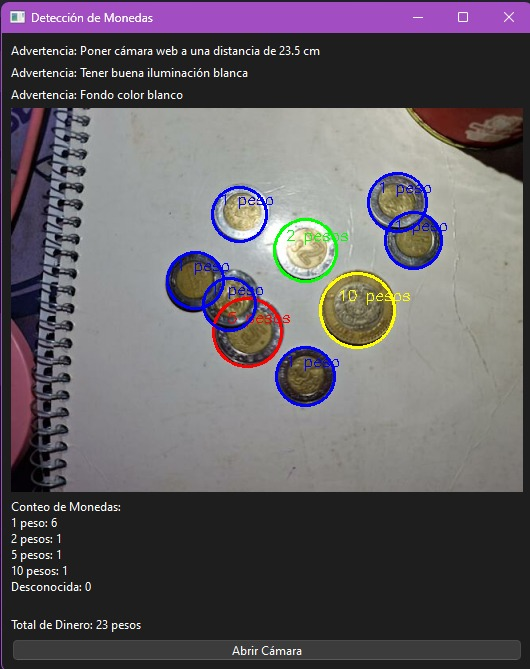
\includegraphics[width=0.32\linewidth]{2024_ConteoMonedasEscritorio/figs/ct2b.jpeg} & 
		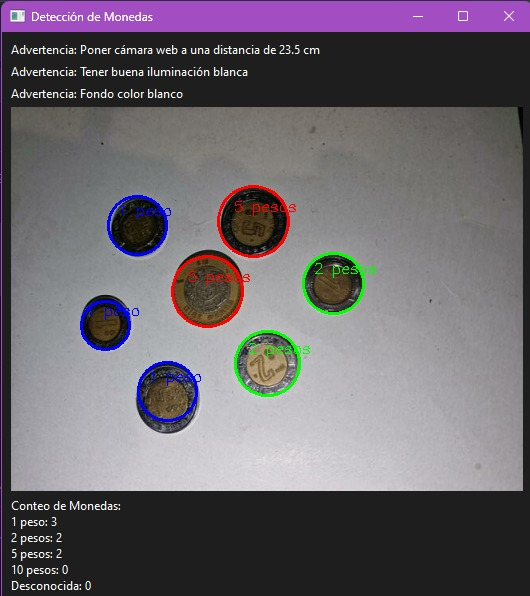
\includegraphics[width=0.36\linewidth]{2024_ConteoMonedasEscritorio/figs/d.jpg}\\
	\end{tabular}
\end{center}

%\column{.1\linewidth}
%\begin{center}%
%	\begin{tabular}{cccc}
%		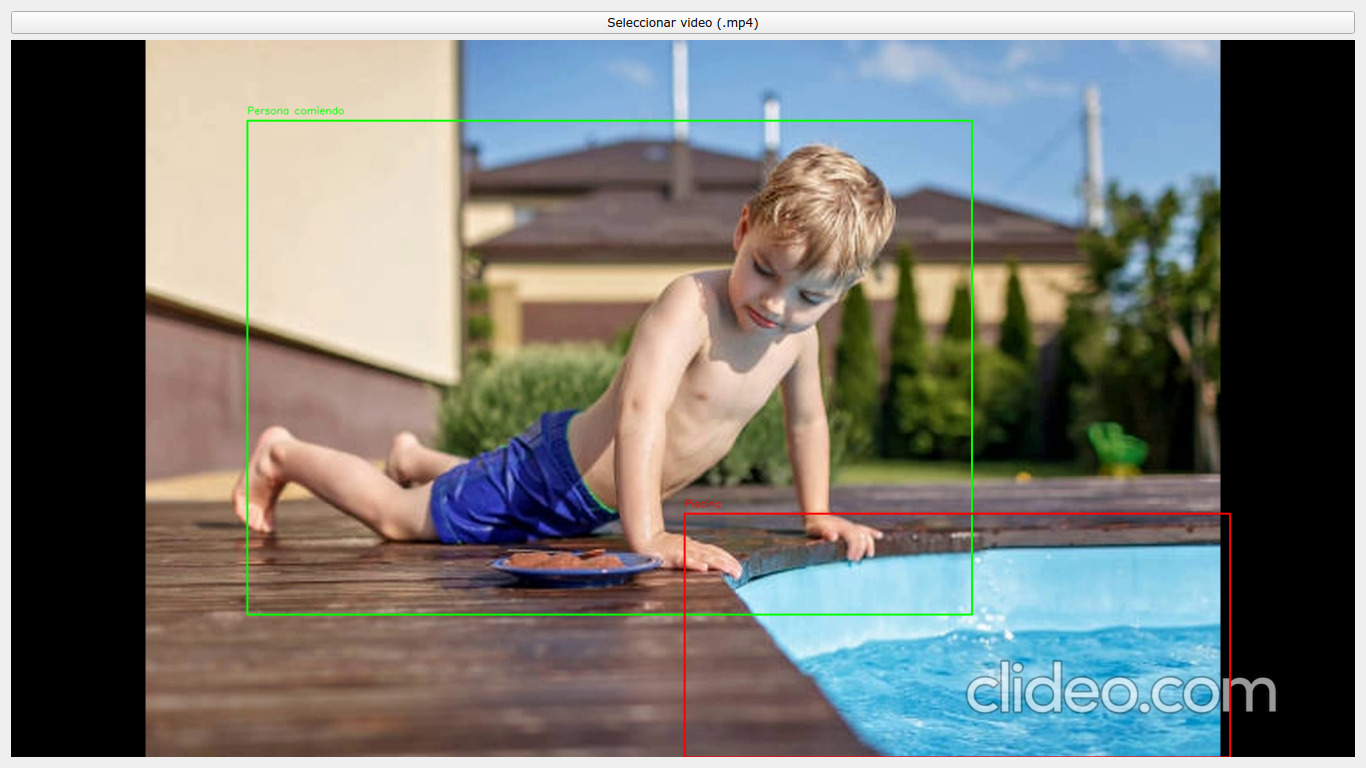
\includegraphics[width=0.48\linewidth]{2024_DeteccionAlimentosAlbercas/figs/im2.jpg} &
 %		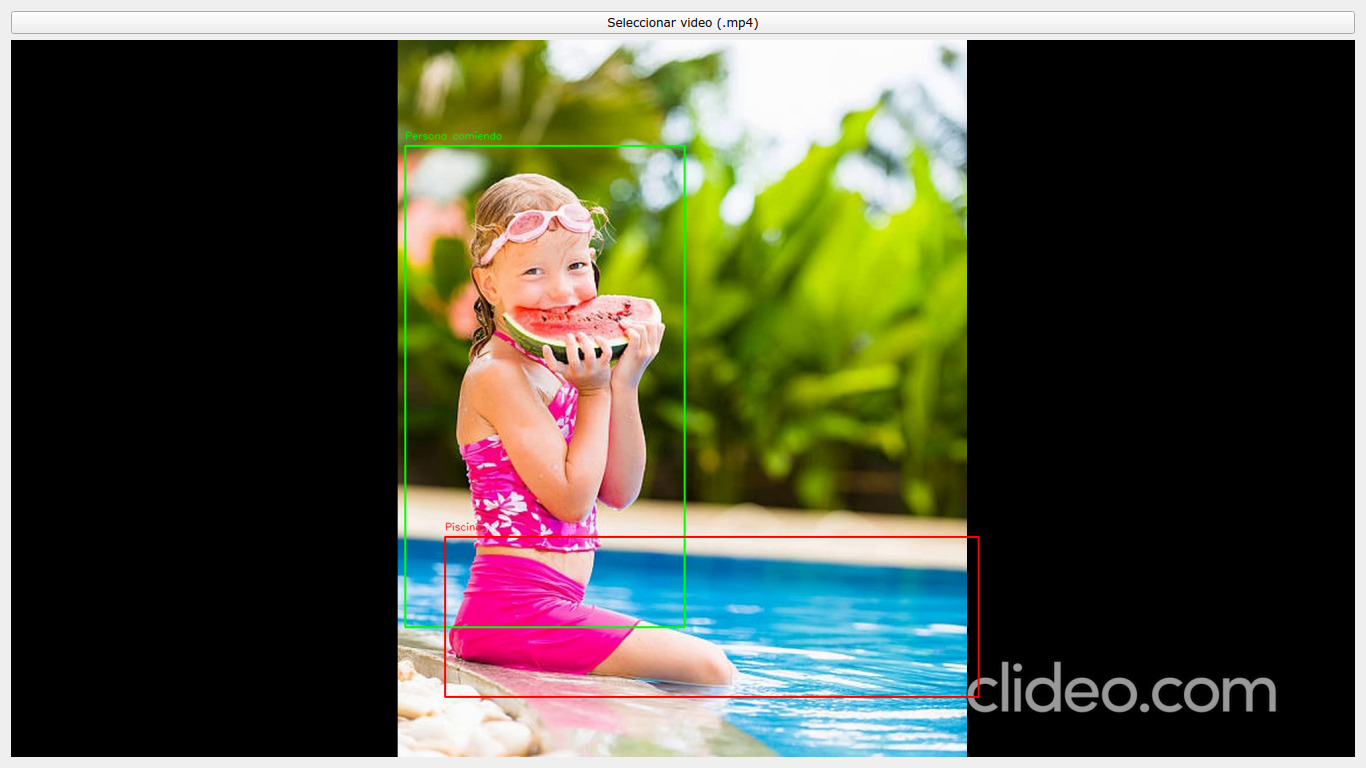
\includegraphics[width=0.48\linewidth]{2024_DeteccionAlimentosAlbercas/figs/im3.jpg} \\
	%	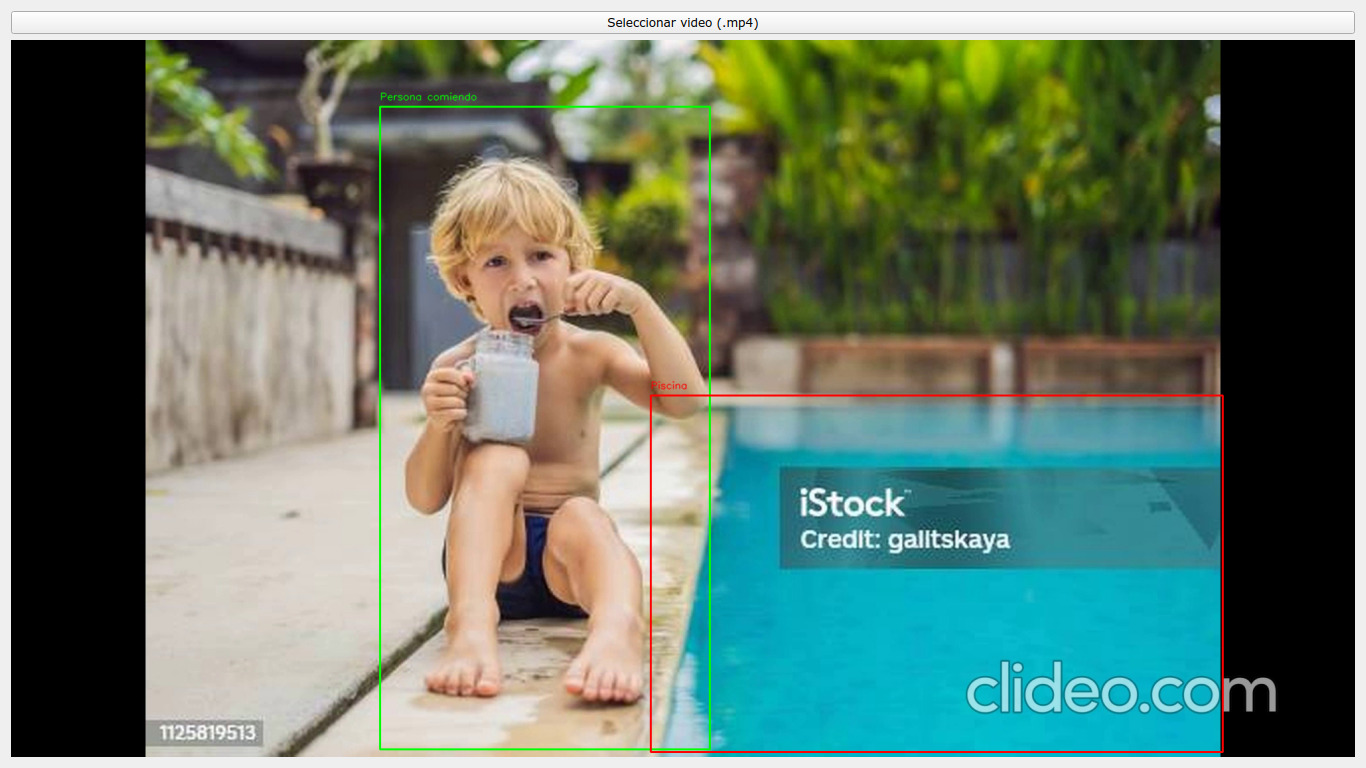
\includegraphics[width=0.48\linewidth]{2024_DeteccionAlimentosAlbercas/figs/im4.jpg} &
 	%	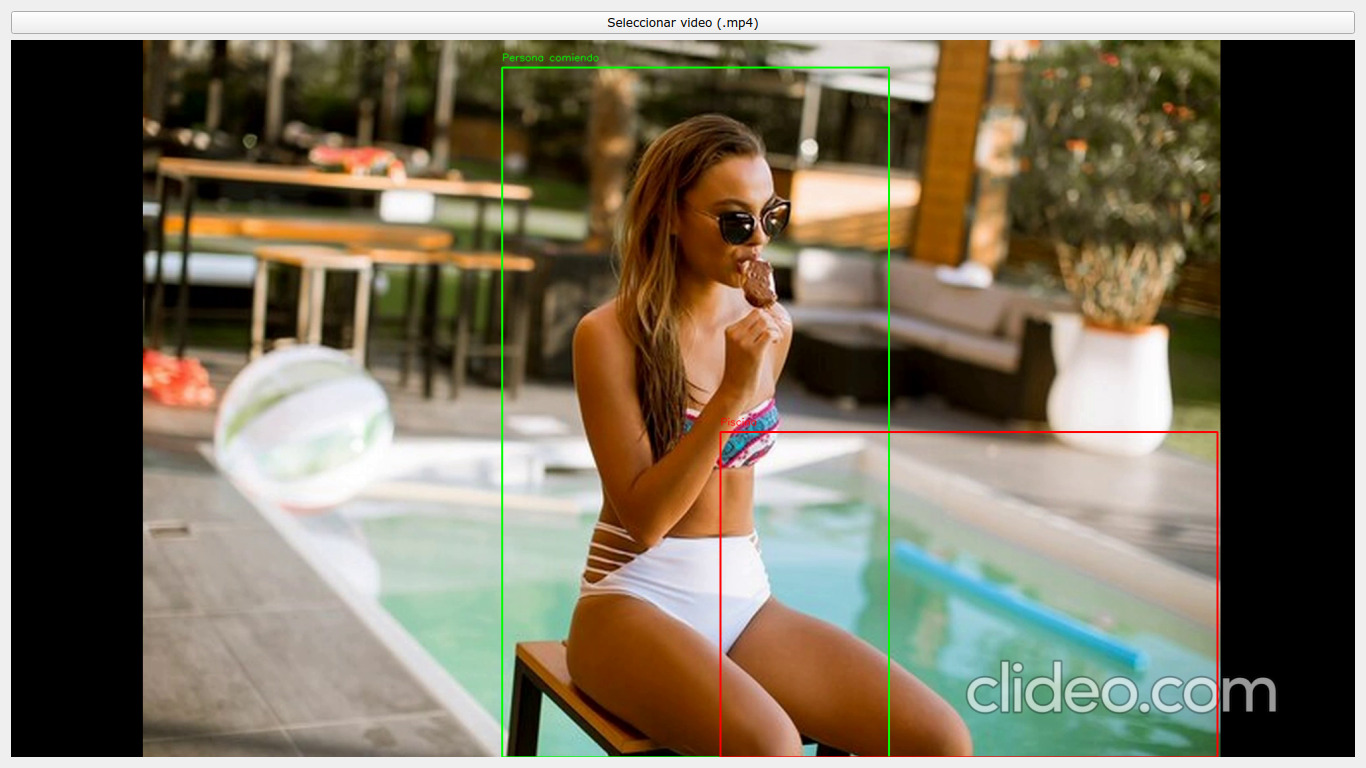
\includegraphics[width=0.48\linewidth]{2024_DeteccionAlimentosAlbercas/figs/im5.jpg} \\
%	\end{tabular}
%\end{center}




%\end{columns}
\end{frame}

%


